\chapter{GATESIM METHODOLOGIES}
\label{chap:methodologies.tex}

Various methodologies are adopted for netlist simulation and verification. For any simulation the first step is getting the test vectors for applying as stimulus to the netlist. One approach is developing a testbench similar to RTL testbench around the netlist and the comparisons are done by this testbench with respect to expected values. Another popular method used is utilizing the test vectors generated for RTL simulation for netlist simulation and comparison done between RTL signal values and gate signal values. 

In AMD gatesim environment, the second approach is adopted where test vectors are obtained from RTL simulation environment. Over the years two different approaches were adopted for test vector access and application. These were Early Dual Sim method and Co-sim Based Gate Sim method. Due to its many disadvantages the early dual sim method was discontinues and currently the co-sim method is the de-facto standard method for gate level simulation.  


\section{EARLY DUAL-SIM METHOD}
 Early method for gate level simulation was a dual-sim or simulation-after- simulation approach. Here RTL simulation was done initially with test bench components. The test vectors for gatesims were generated during this RTL simulation using "\$display" or VCD (value change dump). During the Gatesim, these test vectors were used as stimulus and comparison was done with the RTL output vectors. Figure x shows the simulation flow. ~\figurename{~\ref{fig:earlydualsim.eps}} shows early dual-sim flow.

%\figurename{} 
\begin{figure}[H]
\centering
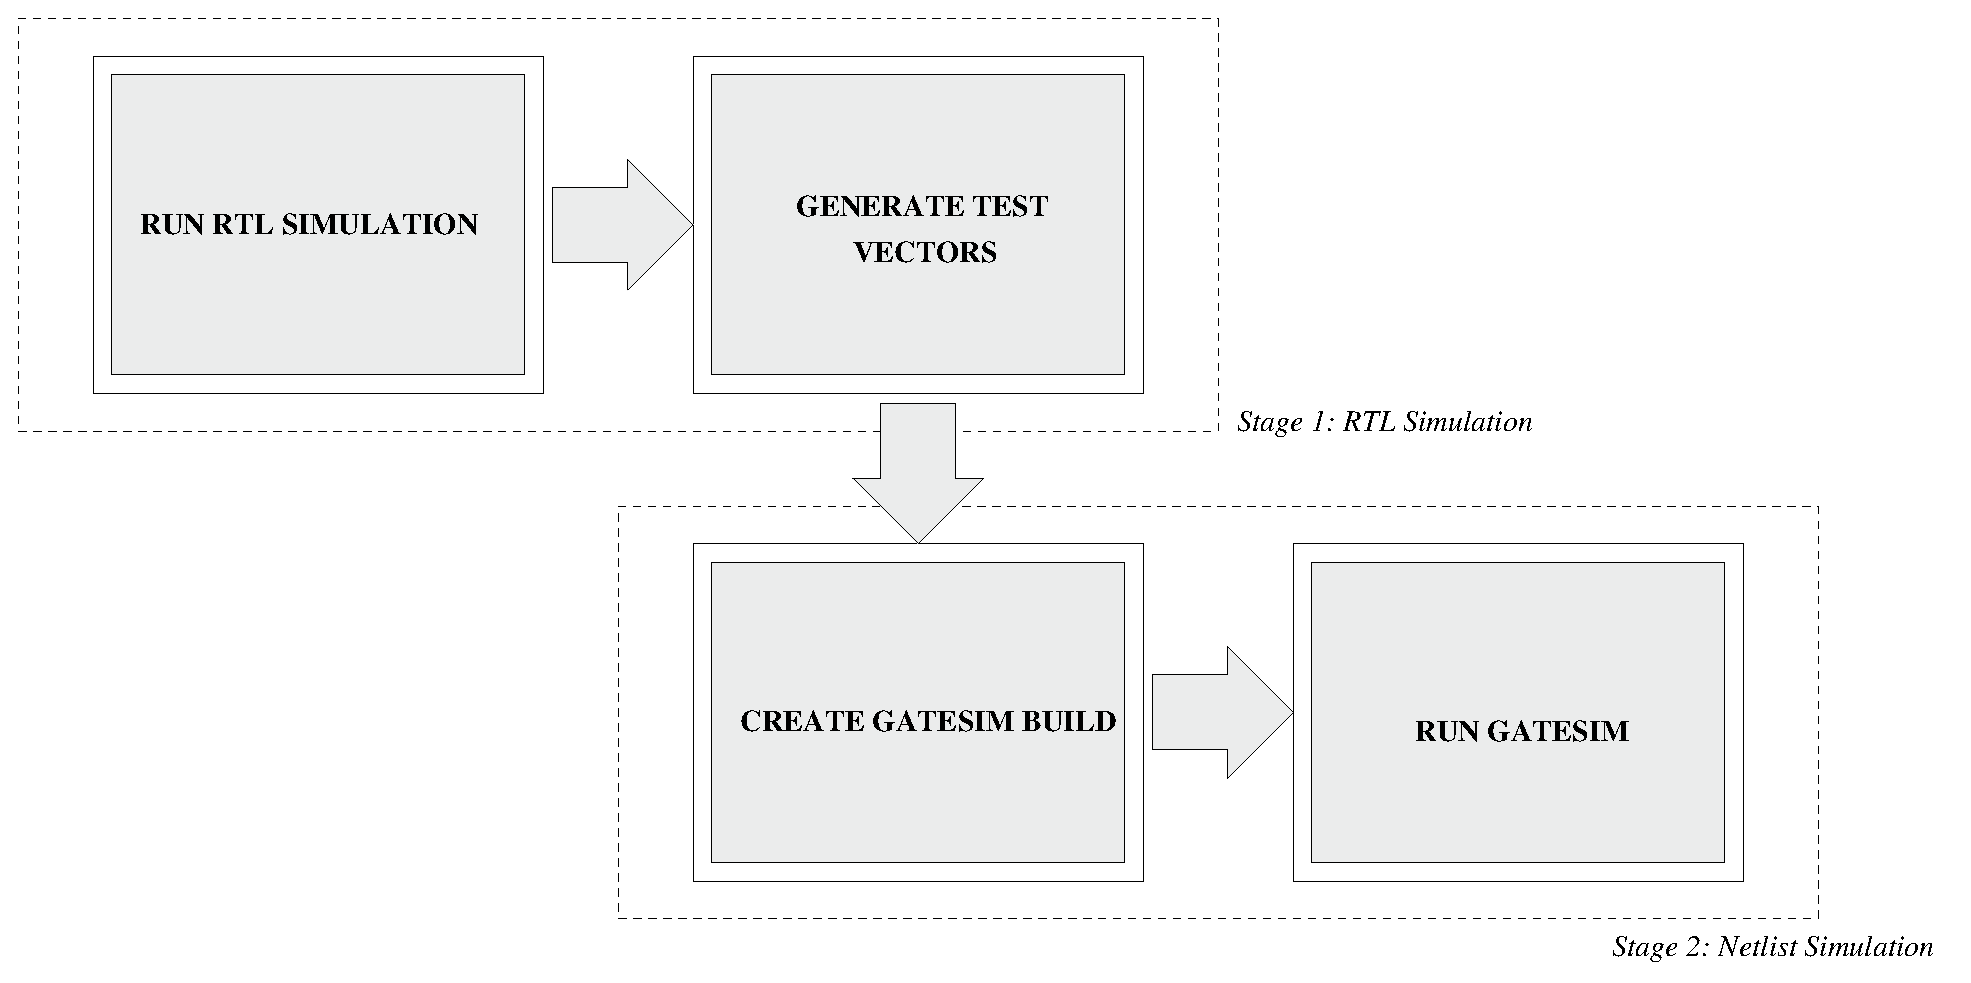
\includegraphics[width=4in, height=3.5in]{./figures/earlydualsim.eps}
\caption{Early Dual-Sim Flow}
\label{fig:earlydualsim.eps}
\end{figure}

This dual- sim approach was widely accepted across industry due to its many advantages. The main advantage of sim after sim is that it had the best simulation performance to memory requirement ratio. However this method had multiple disadvantages which became more evident with increasing design complexity.

\paragraph{Issues:}The main issue with dual sim method used in past was the huge disk space requirement. Vector files were text files which had cycle wise information of stimulus. These files were large and simulation performance was greatly affected due to constant disk input/output accesses. 

 
 With increasing design complexity, the disk-space requirements became too high that the method could no longer sustain and a new co-simulation based approach was adopted instead.





\section{CO-SIM BASED GATESIM}
 Cosim-based approach was conceived to solve some problems that existed with dual-sim approach by allowing easy debug while maintaining common input vectors and output results for comparison.  ~\figurename{~\ref{fig:cosim.ps}} show how stimulus is appiled to netlist and comparison of output is done in co-sim method.
 
\begin{figure}[h!]
\centering
\includegraphics[width=4in, height=3.5in]{./figures/cosim.ps}
\caption{Co-sim Based Gatesim}
\label{fig:cosim.ps}
\end{figure}


 A single combined executable containing the behavioral RTL design, the gate design, and all of the required simulation files is compiled. The behavioral RTL and gate models are run in lock-step with their inputs tied and driven by the testbench and the comparison of the behavioral RTL and gate outputs is done "on the fly". ~\figurename{~\ref{fig:cosim_flow.eps}} shows co-sim flow.




%\figurename{} 
\begin{figure}[H]
\centering
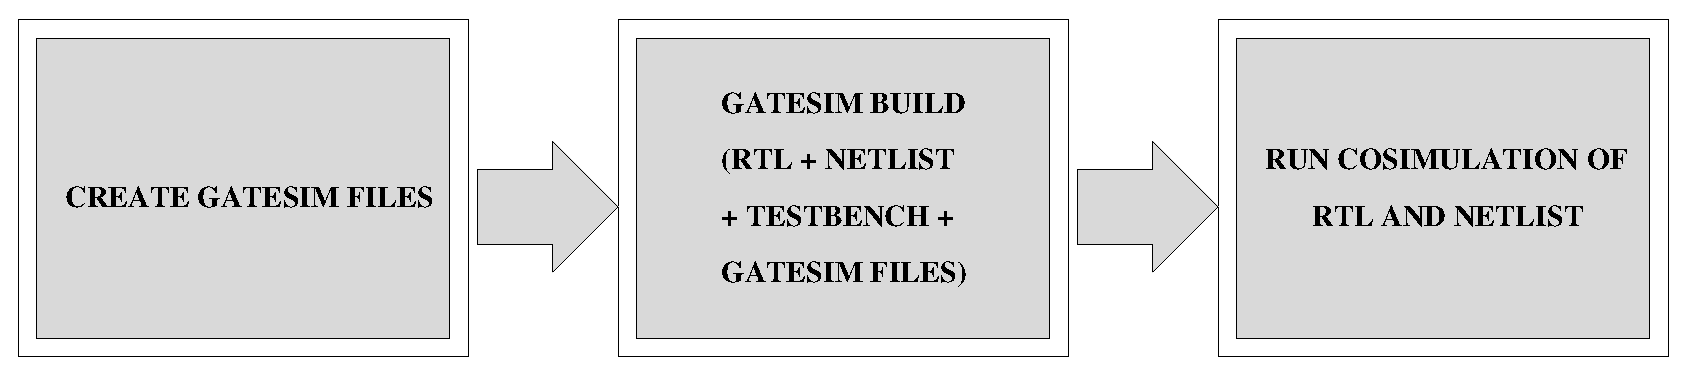
\includegraphics[width=4in, height=1.5in]{./figures/cosim_flow.eps}
\caption{Co-sim Based Gatesim Flow}
\label{fig:cosim_flow.eps}
\end{figure}

Major steps involved in this flow are:

\begin{enumerate}
	\item \emph{\bf Getting gatesim files}

	Input to gatesims are files obtained from LEC tools. These file include the netlist file, files holding information regarding IO/Register mapping, gate defines, compare enables and testbench force files. These inputs from LEC stage are processed by a set of scripts for developing intermediate files which are needed by cosim build infrastructure. These files are called gatesim files and these verilog files are:
	\begin{itemize}
		\item File which contain top level module that connects the behavioral RTL signals to the corresponding gate signals.
		\item Test bench compare files that contain the verilog compare code used to compare the outputs and register mappings.
		\item Force files that contain all the force/release/assign commands for the gates corresponding to RTL force/release/assign statements.
	\end{itemize}

	\item \emph{\bf Getting gatesim build} 

	Next stage is to enable a build structure supporting the co simulation of RTL and Netlist. The build infrastructure will include the following:
	\begin{itemize}
		\item[-]Netlist
		\item[-]RTL
		\item[-]Test bench
		\item[-]Gatesim files
	\end{itemize}

	\item \emph{\bf Run co-simulation of RTL and netlist}

	Finally, run co-simulation. Output files include $<$testname$>$.out which contains the simulation log of the entire test and $<$test name$>$.fsdb (if wave form dump enabled).
\end{enumerate}


As the netlist stimulus is obtained from a live RTL instead if from storage files, co-sim based gatesim overcame the biggest limitation associated with dual-sim. Along with some good set of scripts aiding testbench generation and force generation, this method became the standard method for gatesims ever since.

\subsection {ISSUES WITH CURRENT CO-SIM METHOD}

Co-sim based Gatesim overcame all the known limitation associated with early approach but brought in new set of limitations with ever growing design complexity. Main limitations are:

\begin{itemize}
	\item[-]Larger turn-around time (run, debug cycle).
	\item[-]Limitation on size of netlist (indirect cause due to larger build and run time).
\end{itemize}

\subsubsection {Simulation performance analysis}
Experiments showed that the simulation performance of gatesims was affected sometimes as low as 10\% with respect to its counterpart RTL simulations. This indicates that:

\begin{itemize}
	\item[-]RTL Simulations contribute major to CPS than netlist.
	\item[-]Simulator spends more time in simulating RTL and verification components than netlist.
\end{itemize}

Main causes for this poor simulation performance are:

\begin{itemize}
	\item[-]Test vectors are applied from a live RTL simulation, which runs redundantly for the sole purpose of generating test vectors.
	\item[-]Verification components in modern designs (C, C++, SVTB, OVA, SVA), slow down simulation performance.
\end{itemize}

Evidently it was not an appropriate use of compute resources by having live RTL simulation every time just for the purpose of test vector generation. The analysis provides convincing evidence for us to attempt changes in existing cosim-based methodology.
